%%% ML: text by mel projit kompletni revizi 

%%%%%%%%%%%%%%%%%%%%%%%%%%%%%%%%%%%%%%%%%%%%%%%%%%%%%%%%%%%%%%%%%%%%%%%%%%%%%%%%%%%
%%                 PŘÍLOHA - UŽIVATELSKÁ PŘÍRUČKA                                %%
%%%%%%%%%%%%%%%%%%%%%%%%%%%%%%%%%%%%%%%%%%%%%%%%%%%%%%%%%%%%%%%%%%%%%%%%%%%%%%%%%%%
\chapter{User guide}
\label{user-guide}

%%% ML: works with -> usage of the plugin can change accross...
This user guide is written for plugin using in QGIS 2.12. There is a~possibility that usage of the plugin
can change across other versions of QGIS. 

\section{Loading of plugin}
\label{plugin-load}

There are many ways to install the~plugin.
The~easiest method is to install it from
the~QGIS Plugin repository. 

Firstly, you have to open the~plugins dialog – select
\textit{Manage and install plugins} from
\textit{Plugins} tab. Plugin is now registered as
experimental, to see it select \textit{Settings}
tab and tick the~checkbox \textit{Show also experimental plugins}. 

%  \begin{figure}[H]
%   \centering
%	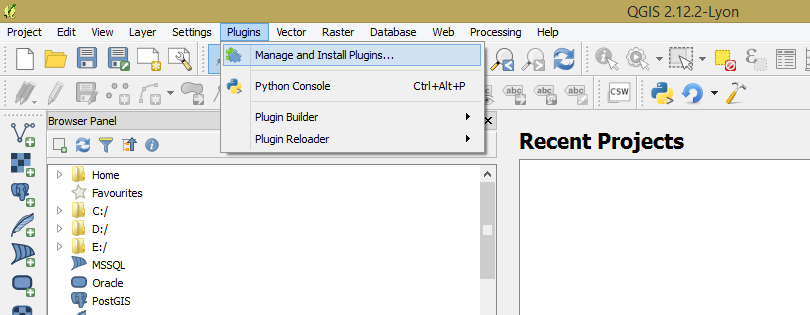
\includegraphics[scale=0.1]{./pictures/plugin-tab.png}
%	\caption[GUI]{Plugins tab}
%      \label{fig:plugins-tab}
%  \end{figure}

Search for \textit{GPS Position Lag Correction} plugin in
the~list on the~\textit{All} or \textit{Not installed} tab.
Select it and press the~\textit{Install} button. 

  \begin{figure}[H]
   \centering
	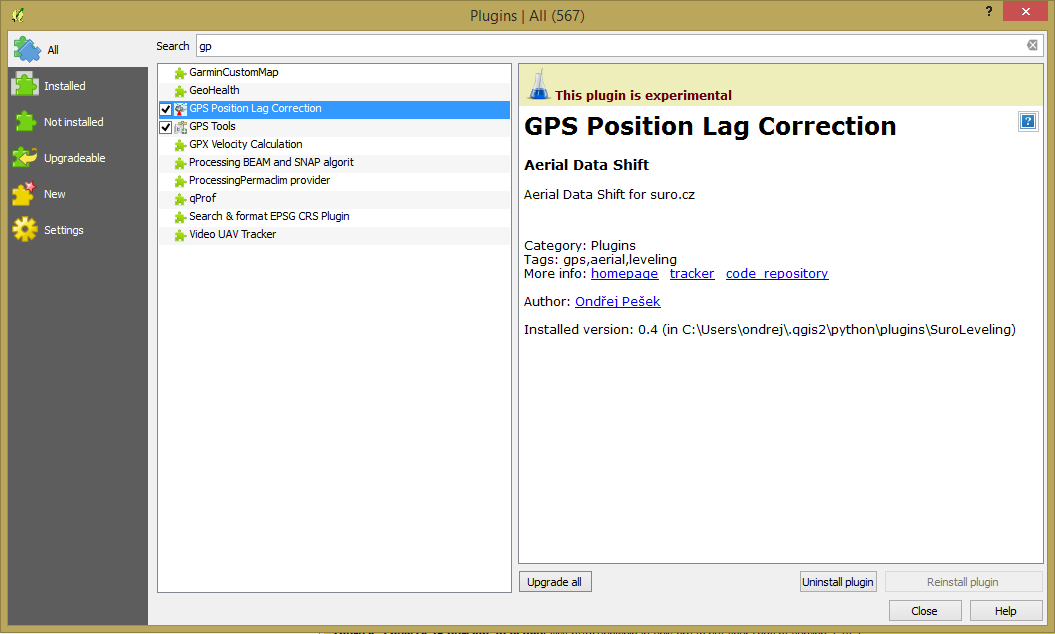
\includegraphics[scale=0.52]{./pictures/plugin-dialog.png}
	\caption[GUI]{Plugins dialog}
      \label{fig:plugins-dialog}
  \end{figure}

\section{Work with plugin}
\label{work}

%%% ML: preformulovat In this section will be described graphical user
%%% interface and primary functionality of the plugin
In this section will be described graphical user interface and primary functionality of the plugin. 

  \begin{figure}[H]
   \centering
	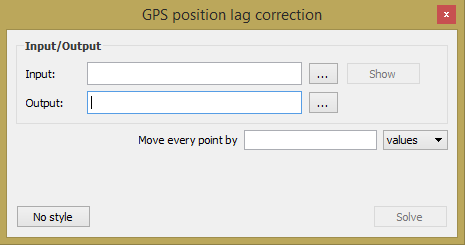
\includegraphics[scale=0.75]{./pictures/gui.png}
	\caption[GUI]{GUI of the plugin}
      \label{fig:gui}
  \end{figure}

\subsection{Input and output defining}
\label{input-output}

As input, you have to define the~file you want to work
with. You can write the~path to this file manually or
there is the~button with \Fbox{ ... }. By clicking
on this button, you will get the~dialog intended to
choose your file. Click on OK will insert this path
to the~basic interface. Click
on Cancel will interrupt the~choosing dialog,
and the~input path will not be changed. 

  \begin{figure}[H]
   \centering
	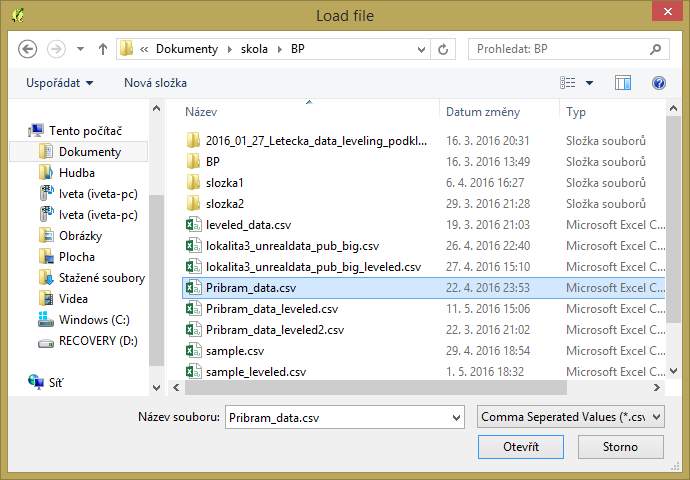
\includegraphics[scale=0.75]{./pictures/input.png}
	\caption[Loading input]{Loading input}
      \label{fig:input}
  \end{figure}

The~same procedure is with output, but there you define
the~path where the~new file will be created.
The~choosing dialog for output is intended to
choose folder, not file. 

 \begin{figure}[H]
   \centering
	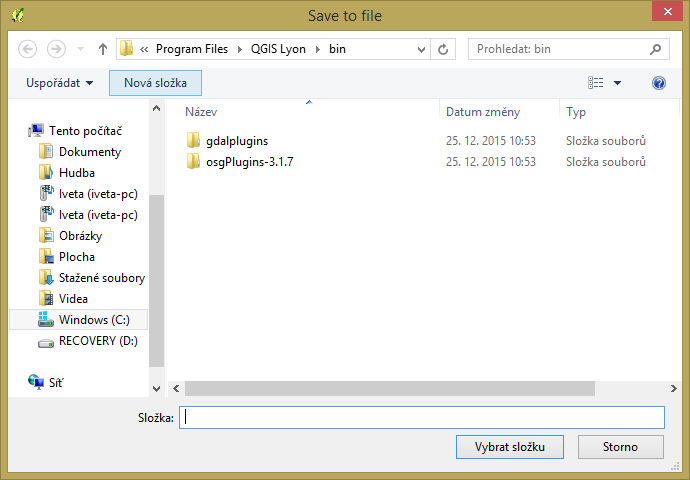
\includegraphics[scale=0.75]{./pictures/output.png}
	\caption[Choosing output directory]{Choosing output directory}
     \label{fig:output}
  \end{figure}

\subsection{Styling}
\label{styling}

There is also optional possibility of styling your points for better visualisation. 

By default, you have not defined any style
and points will be created in default QGIS style
(on Style button is written \textit{No style})
If you want your own style, you have to click on
this button. You will get the~browsing dialog.
You are automatically directed to folder
\textit{styles} in the~plugin folder; here you can
choose qml file and click OK. Click on Cancel
interrupts the~dialog and set again \textit{No style}. 

If you choose your own style, you will see its name on the~style button. 

In the~default version of plugin there are two presetted styles. Styling in those styles is based on
column {\tt mereni} – one style for higher and one style for lower values. 

  \begin{figure}[H]
   \centering
	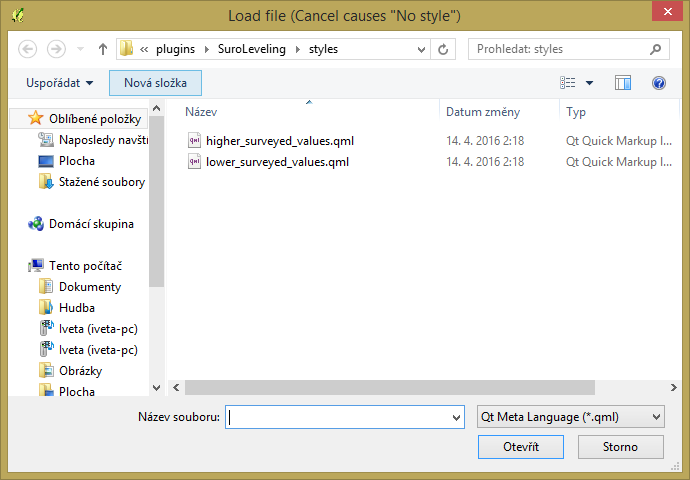
\includegraphics[scale=0.75]{./pictures/style.png}
	\caption[Choose style]{Choose style}
      \label{fig:style}
  \end{figure}

  \begin{figure}[H]
   \centering
	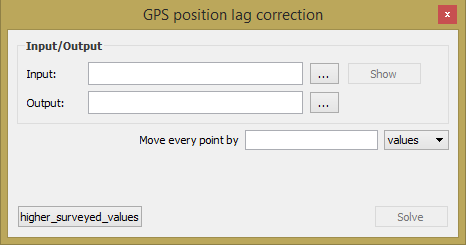
\includegraphics[scale=0.75]{./pictures/style-defined.png}
	\caption[Used style]{Used style}
      \label{fig:used-style}
  \end{figure}

\subsection{Showing input}
\label{show}

Next to input is the~button \textit{Show}. 

Show button is just to visualise the~input file as layer in QGIS. It has no effect on the~run of plugin
and it is not necessary for it, but it allows you to visualise the~input file in the~same style as
the~output file. It gives you also the~opportunity to compare the~shifted values with the~original ones. 

This button was created on request by users who prefer to visualise both the~input and the~output from
one dialog. 

If input file does not exist, the~plugin raises the~error message. 

%%% ML: Shift
\subsection{Shift}
\label{shift}

Shift will be done by clicking on button \textit{Solve}.
Before shifting you have to define some proprieties. 

In combo box (drop-down list) you can choose the~units of
shift – each presents other type of shift; values mean shift
by values, meters mean shift by constant distance and seconds
mean shift by constant time/variable
distance considering current velocity. 

%%% ML: nepouzivat lineedit v textu
In the~appropriate line text editor you have to insert
value of move. For shift by values it should be integer (it
does not make sense to shift point by 1.5 values because
nothing like 1.5 value does not exist), for
other shifts it should be integer or float. 

For wrong input, plugin raise the~error message. 

\subsection{Dependencies}
\label{dependencies}

To avoid some unnecessary errors, there are some dependencies in the~plugin graphical nterface. 

The~first is \textit{Show} button. This button is
disabled until you have wrote anything into input. 

  \begin{figure}[H]
   \centering
	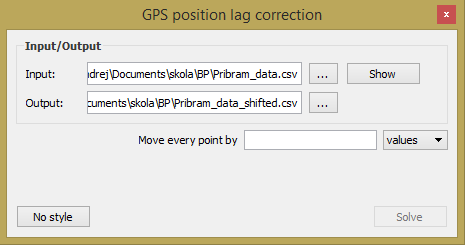
\includegraphics[scale=0.75]{./pictures/show.png}
	\caption[Enabled Show button]{Enabled Show button}
      \label{fig:show}
  \end{figure}

The~second is button \textit{Solve}. You can’t solve anything until you have defined input, output and
value of shift.

  \begin{figure}[H]
   \centering
	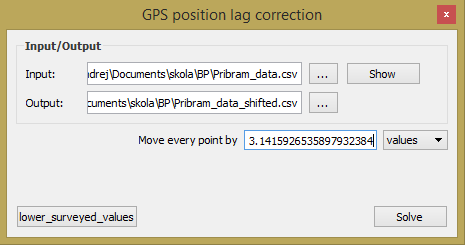
\includegraphics[scale=0.75]{./pictures/solve.png}
	\caption[Enabled Solve button]{Enabled Solve button}
      \label{fig:solve}
  \end{figure}

There is also implemented a~shortcut for defining output
directory. Many users want to save output file to
the~directory from which was read the~input file;
so when you choose input file, the~directory will
be automatically copied into output,
just with added \textit{\_shifted} into filename. 
